\documentclass[12pt]{article}

\usepackage[utf8]{inputenc}
\usepackage[russian]{babel}
\usepackage{geometry}
\usepackage{graphicx}
\usepackage{soul}
\usepackage{color}
\usepackage{colortbl}

\geometry{a4paper, top=15mm, bottom=15mm, left=10mm, right=10mm}

\begin{document}

\setcounter{page}{0}
\thispagestyle{empty}

\begin{center}
    Федеральное государственное автономное учебное учреждение высшего образования\\
    <<Национальный исследовательский университет ИТМО>>\\
\vspace{0.5cm}
    Мегафакультет компьютеных технологий и управления\\
    Факультет программной инженерии и компьютерной техники
\end{center}

\vspace{3cm}

\begin{center}
\Large
\textbf{
    Отчёт\\
    по лабораторной работе №3\\
    по дисциплине <<Программирование>>
}
\end{center}

\begin{center}
\large
    Вариант 31180120.5
\end{center}

\vspace{6cm}

\begin{flushright}
    Студент: Кожухин Иван Алексеевич, группа P3118\\
    Преподаватель: Письмак Алексей Евгеньевич
\end{flushright}

\vspace{6cm}

\begin{center}
    Санкт-Петербург\\
    2022
\end{center}

\newpage

\tableofcontents

\newpage

\section{Задание}

По заданной предметной области построить объектную модель. Программа должна удовлетворять следующим требованиям:\\
1. Доработанная модель должна соответствовать принципам SOLID.\\
2. Программа должна содержать как минимум два интерфейса и один абстрактный класс (номенклатура должна быть согласована с преподавателем).\\
3. В разработанных классах должны быть переопределены методы equals(), toString() и hashCode().\\
4. Программа должна содержать как минимум один перечисляемый тип (enum).\\
Порядок выполнения работы:\\
1. Доработать объектную модель приложения.\\
2. Перерисовать диаграмму классов в соответствии с внесёнными в модель изменениями.\\
3. Согласовать с преподавателем изменения, внесённые в модель.\\
4. Модифицировать программу в соответствии с внесёнными в модель изменениями.\\
Текст задания варианта:\\
\textit{<<Отправившись с гостем на кухню, Спрутс разломал пару стульев и растопил печь, после чего расколотил яйцо, но, вместо того чтоб выпустить его на сковородку, выпустил его на собственные штаны. Решив, что если дело пойдет так дальше, то ему вовсе не придется поужинать, Жулио отнял у Спрутса яйца и принялся за дело сам. Выбрав сковороду побольше, он соорудил гигантскую яичницу из двух десятков яиц, и они со Спрутсом уселись ужинать. Спрутс ел и только похваливал, так как ему уже давно не приходилось есть так хорошо приготовленную яичницу. Сообразив, что Жулио может оказаться для него полезен, поскольку мог бы ходить за продуктами и помогать готовить обед, Спрутс предложил ему поселиться вместе. Жулио согласился, и с тех пор жизнь Спрутса приобрела более организованный характер. Доставку продуктов из магазинов Жулио целиком взял на себя, завтраки же, обеды и ужины они готовили вместе, причем Спрутс производил более грубую работу, то есть "делал" дрова из мебели, разжигал огонь в топке, чистил картошку, лук, репу, месил тесто; Жулио же осуществлял общее руководство и следил за качеством изготовляемых блюд. Кроме заботы о пище, Жулио проявил также заботу о чистоте. Поскольку топить лишний раз печь им было лень, а по ночам бывало зябко, Жулио придумал спать не на кроватях, а в сундуках. Забравшись вместе с периной в сундук и закрывшись в нем крышкой, можно было согреть дыханием воздух и спать, не ощущая холода. В те времена как для господина Жулио, так и для господина Спрутса самым большим удовольствием было усесться вечерком, после дневных забот, у телевизора и начать проклинать новые порядки. По телевидению тогда часто показывали рабочих, которые теперь самостоятельно, без господ управляли своими фабриками и заводами. Особенный интерес представляло то, что многие производственные процессы протекали теперь в состоянии невесомости. Господин Спрутс и господин Жулио невольно подсчитывали, какие выгоды могли бы иметь богачи, если бы невесомость досталась им, а не рабочим, и это прямо-таки выводило их из себя. Но больше всего выводили их из себя разговоры о гигантских растениях, которые и на самом деле росли не по дням, а по часам. Не проходило дня, чтоб по телевидению теперь не показывали зреющих гигантских огурцов, помидоров, капусты, свеклы, арбузов, дынь, которые к тому же были посажены на землях, отобранных у богачей. И Спрутсу и Жулио становилось не по себе, когда они видели высоченные колосья наливающейся земной пшеницы. Однажды диктор объявил, что скоро будет передача из Космического городка, который построили прилетевшие космонавты. Спрутс и Жулио едва усидели на стульях, до того им не терпелось поскорей увидеть своих врагов. Наконец на экране появился Знайка. Он представил телезрителям своих друзей-космонавтов, с которыми прилетел на Луну, показал несколько маленьких уютных домиков, которые космонавты построили для себя сами. Зрители даже увидели один такой домик внутри. Потом были показаны различные научные приборы, и Фуксия рассказала о той научной работе, которая проводилась космонавтами на Луне. Тюбик показал лунатикам несколько земных пейзажей, которые он нарисовал тут же, и рассказал, чем отличается жизнь на Большой Земле от жизни на Луне. После него выступил Гусля, который сыграл на флейте несколько мелодий, чтоб познакомить лунатиков с музыкой, которая в ходу у земных коротышек.>>}

\newpage

\section{Ход работы}

Исходники кода программ и файлов:\\
\\
\textbf{https://github.com/troublegale/ProgLab4}

\begin{figure}[h]
    \centering
    
\includegraphics{image1.png}
    \caption{QR-код для доступа к репозиторию на GitHub}
\end{figure}

\begin{figure}[h]
    \centering
    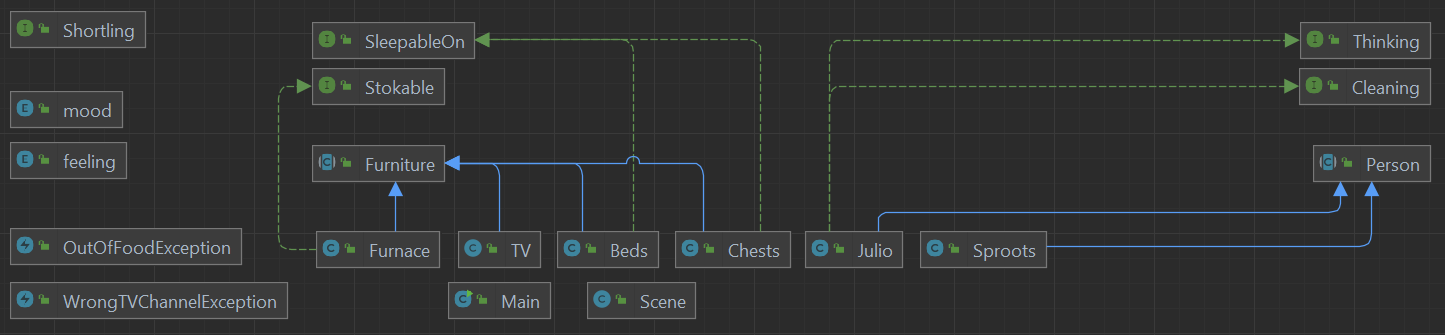
\includegraphics[width=0.8\linewidth]{image2.png}
    \caption{Диаграмма классов объектной модели}
\end{figure}

\begin{figure}[h]
    \centering
    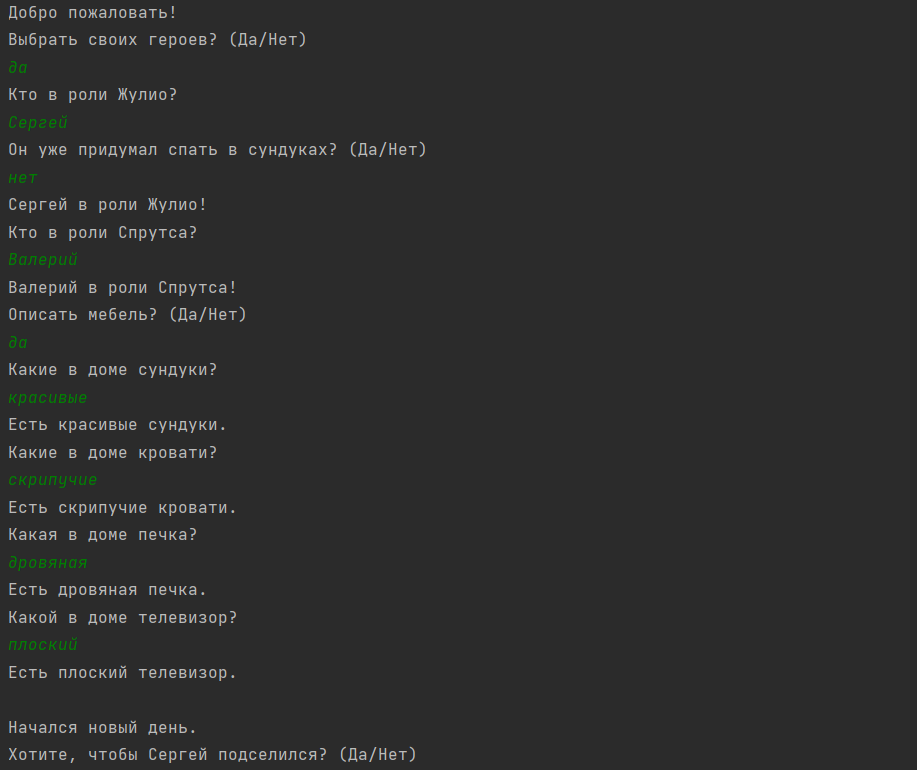
\includegraphics[width=0.52\linewidth]{image3.png}
    \caption{Пример вывода программы, часть 1}
\end{figure}
\newpage
\begin{figure}[h]
    \centering
    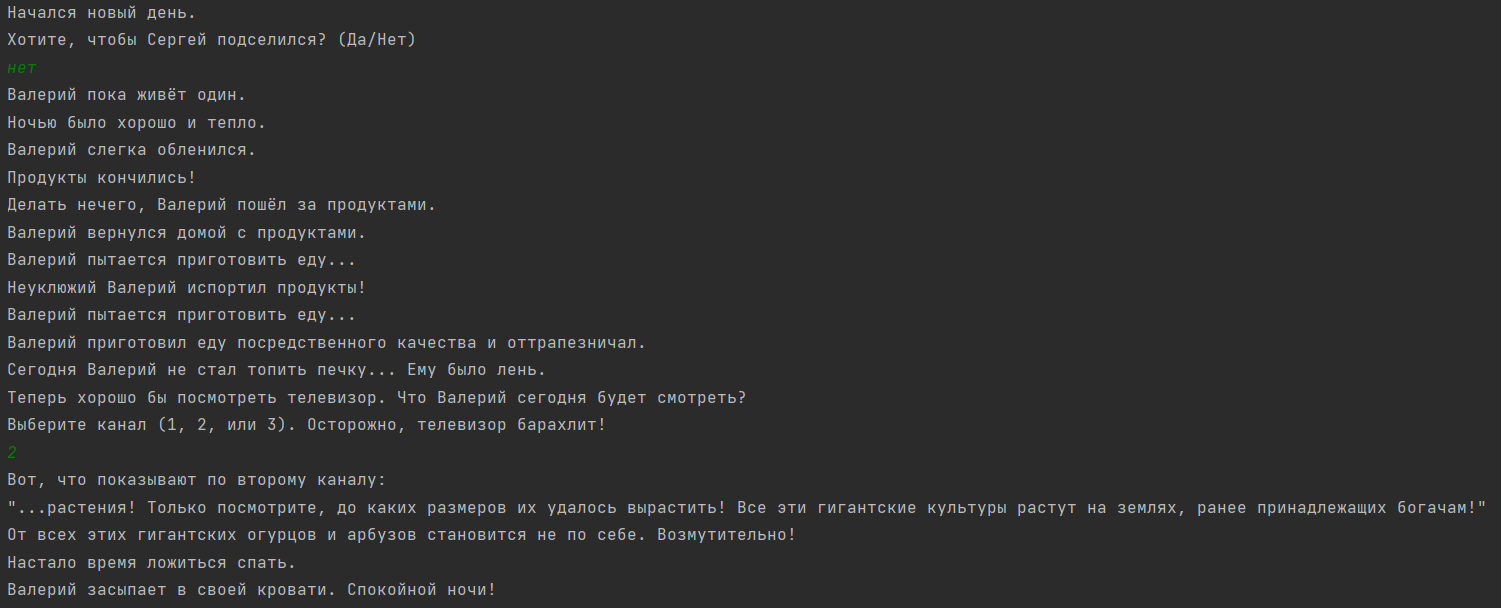
\includegraphics[width=\linewidth]{image4.png}
    \caption{Пример вывода программы, часть 2}
\end{figure}

\begin{figure}[h]
    \centering
    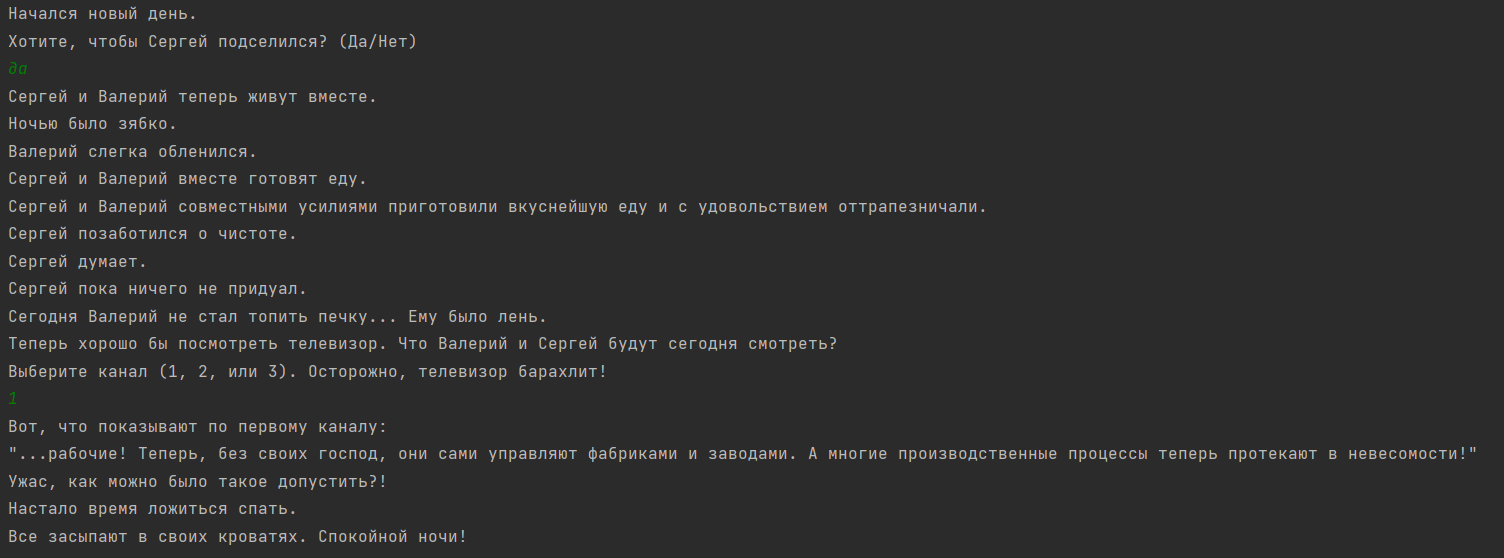
\includegraphics[width=\linewidth]{image5.png}
    \caption{Пример вывода программы, часть 3}
\end{figure}
\newpage
\begin{figure}[h]
    \centering
    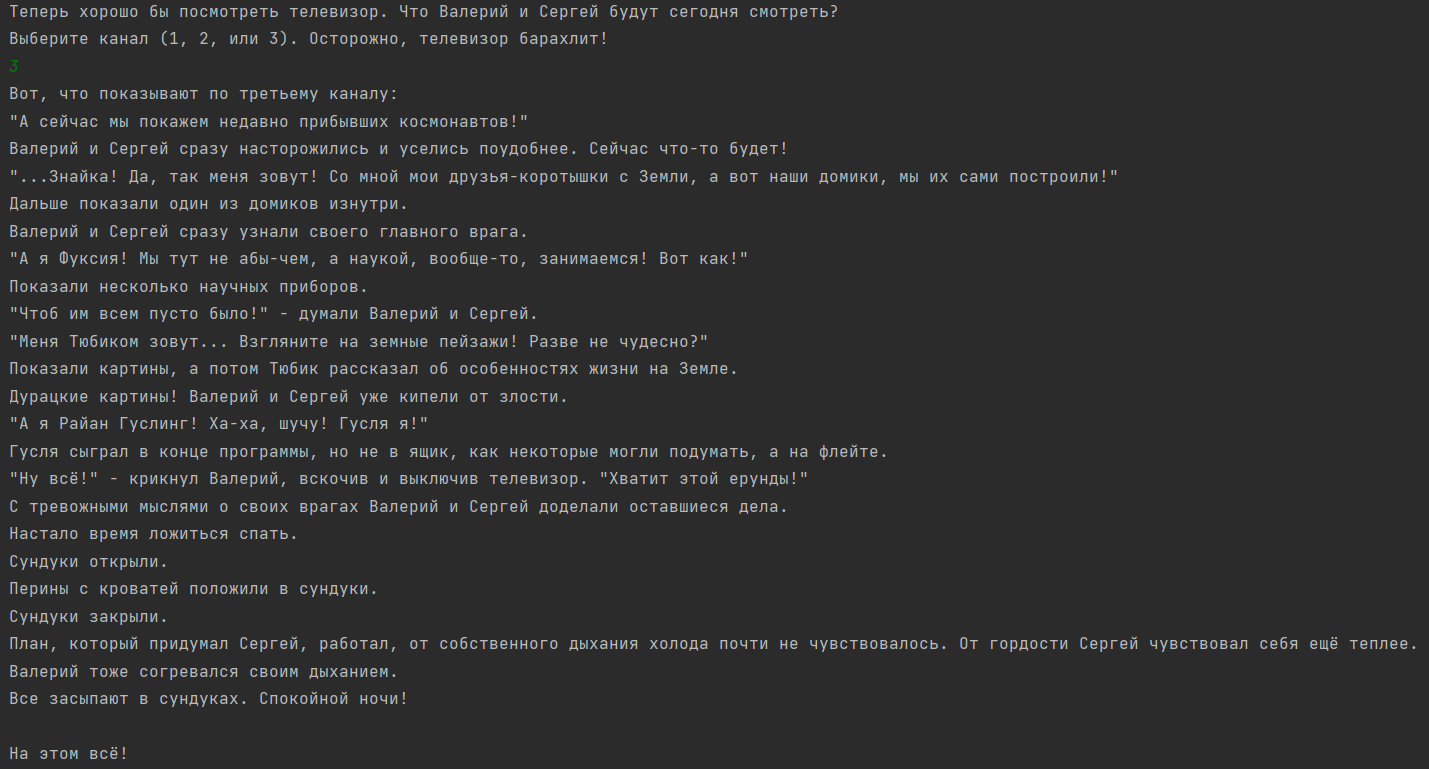
\includegraphics[width=\linewidth]{image6.png}
    \caption{Пример вывода программы, часть 4}
\end{figure}

\begin{figure}[h]
    \centering
    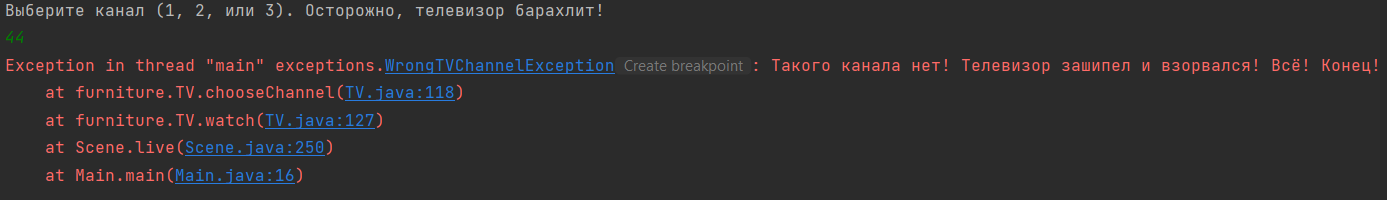
\includegraphics[width=\linewidth]{image7.png}
    \caption{Пример вывода исключения}
\end{figure}
\newpage

\section{Вывод}

В ходе лабораторной работы я закрепил знания о принципах SOLID и ООП на языке Java, доработал объектную модель по расширенному описанию, узнал о видах исключений и классов в Java.

\end{document}